\chapter{Results} \label{chapter:results}

% 논문의 목적에 따라 실행한 연구 결과를 부제에 맞추어 기술하고 구체적인 데이터를 그림이나 표로 제시한다.

\section{Effect of Space Optimization}

The effect of space optimization for k-mer table and ID table is visualized in the \autoref{fig:space_opt}.
For the forementioned 900MB database in \cref{section:space-optimization}, \autoref{fig:k11_space}, when we generate \texttt{Petasearch} data structures for 11-mers, the total space usage is reduced from 17.8GB to merely 849MB (0.85GB), decreasing the space usage by $95.35\%$ compared to the original \texttt{Petasearch} data structures.
Viewing separately, the space usage of the k-mer table is reduced from 5.9GB to 405MB ($-93.34\%$), and the space usage of the ID table is reduced from 11.9GB to merely 444MB ($\-96.36\%$).
The effect of ASCII-squeezing method and simplified database index combined is exhibited in \autoref{fig:ascii-squeezing}.
The size of the sequence database was reduced by $28.27 \%$ for a 300MB-scale database.
For gigabyte-sized database, the compression efficiency is even higher -- a 82.1GB database got compressed to only 46.3GB thanks to ASCII-squeezing method and simplified index.

\section{Speed Benchmark}

Because of space limitation, the detailed effect of each optimization was omitted. Instead we present the results of speed benchmark in \autoref{tab:time_benchmark} with all optimizations applied. The results were also visualized in visualized in \autoref{fig:speed} to give the readers an intuitive impression of how fast the algorithm is. It is noteworthy that in the benchmark for \texttt{Petasearch} prototype, the searching time for a 456GB target set was already 15m 49s without generating similar k-mers. Using the same algorithm with the same parameters, the searching time for a 456GB target set is currently only 3m32s, suggesting that the algorithm is now 5 times faster than the prototypical implementation.

\section{Sensitivity Benchmark}

We visualized the sensitivity benchmark in \autoref{fig:sensitivity}. It is confirmed that \texttt{Petasearch} worked as expected as it found a similar number of high sequence identity hits to other methods. The performance is comparable up to $60\%$ sequence identity. Moreover, it is also clearly shown that \texttt{Petasearch}'s profile search mode have similar performance as \texttt{MMseqs2}'s profile search, enabling \texttt{Petasearch} to capture true positive hits at sequence identity as low as $40\%$. The integration of profile search function is proved to be successful, bringing the applicability of \texttt{Petasearch} to a new level.

\pagebreak
\begin{figpage}
  \newgeometry{left=8mm, right=10mm, top=20mm}
  \captionsetup[figure]{width=.9\linewidth}
  \captionsetup[subfigure]{
    width=.9\linewidth
  }
  \centering
  \begin{figure}
    \begin{subfigure}{0.5\textwidth}
      \centering
      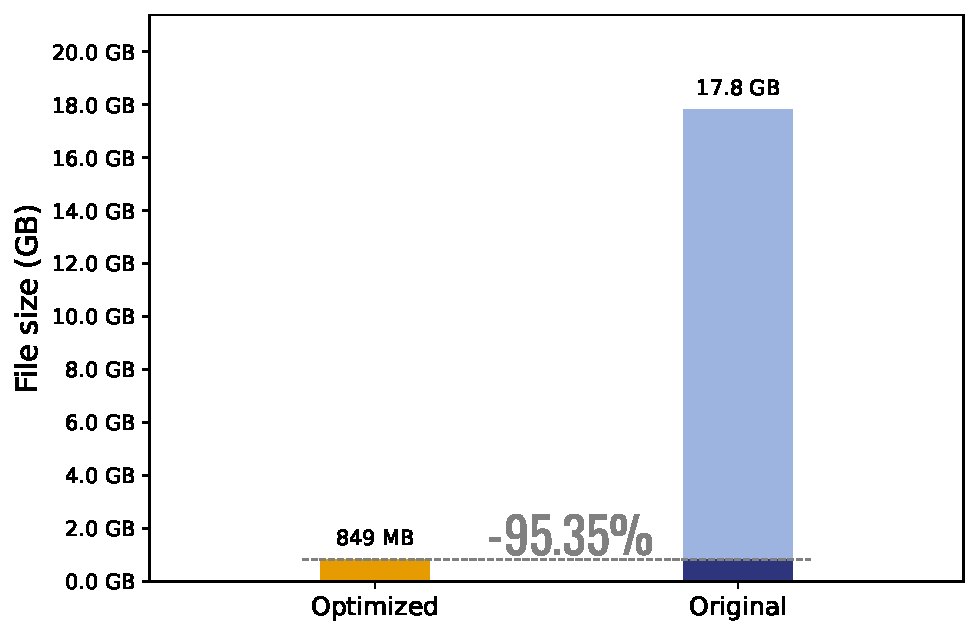
\includegraphics[width=\textwidth]{images/bitsqueeze_alternative.pdf}
      \centering
      \caption{Visualization of he total amount of reduction in space usage for the \texttt{Petasearch} data structures.
        The great reduction in space usage makes the previous implausible search for 11-mer index possible.}
      \label{fig:total_effect_of_bitsqueeze}
    \end{subfigure}
    \begin{subfigure}{0.5\textwidth}
      \centering
      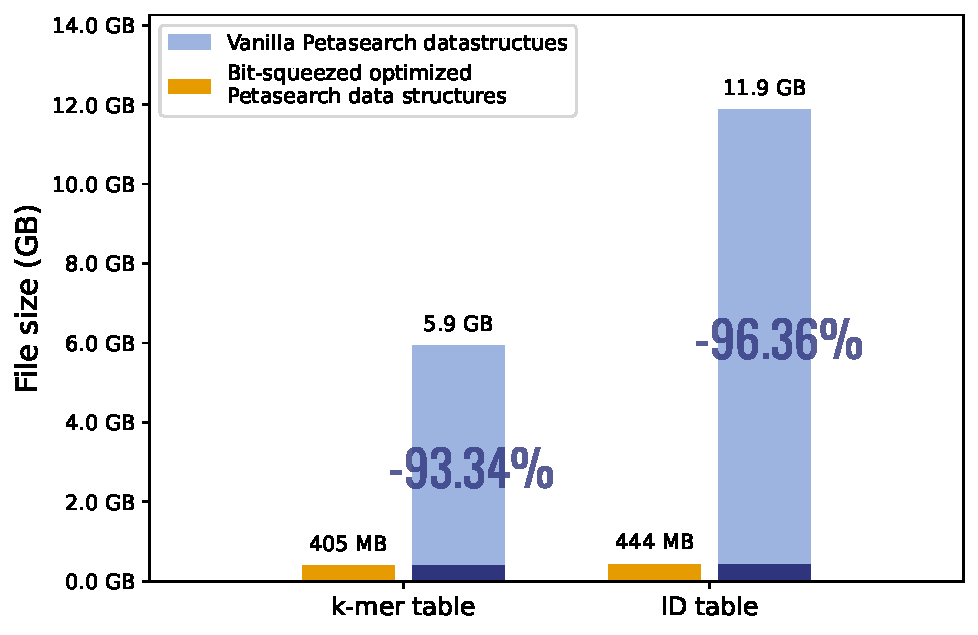
\includegraphics[width=\textwidth]{images/bitsqueeze_optimization.pdf}
      \caption{Visualization of the space reduction for k-mer table and ID table separately.
        The carefully designed bit-squeezing technique and redundancy reducion for ID table are both highly effective.}
      \label{fig:separate_effect_of_bitsqueeze}
    \end{subfigure}
    \caption{\textbf{Effect of space optimization for k-mer diff-index table and ID table using bit-squeezing technique at $\mathbf{k = 11}$.} \cref{fig:total_effect_of_bitsqueeze} showed the total effect of bit-squeezing on both \texttt{Petasearch} data structures.
      \cref{fig:separate_effect_of_bitsqueeze} showed the effect of bit-squeezing on the k-mer diff-index table and the ID table separately.}
    \label{fig:space_opt}
  \end{figure}
  \begin{figure}
    \begin{subfigure}{0.5\textwidth}
      \centering
      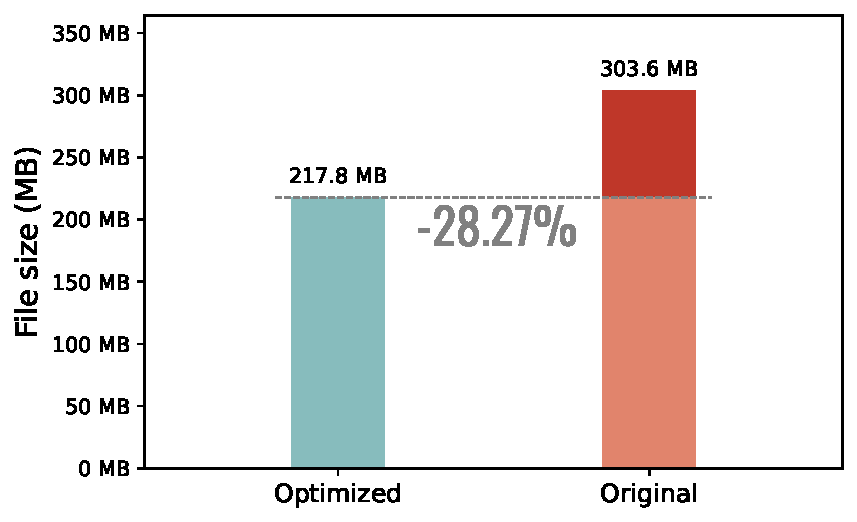
\includegraphics[width=\textwidth]{images/seqdbsize_small.pdf}
      \caption{The amount of space reduction for a 303.6 MB database. The space saving is about $28.27\%$ or one third of the size of the original database.}
      \label{fig:seqdbsize_small}
    \end{subfigure}
    \begin{subfigure}{0.5\textwidth}
      \centering
      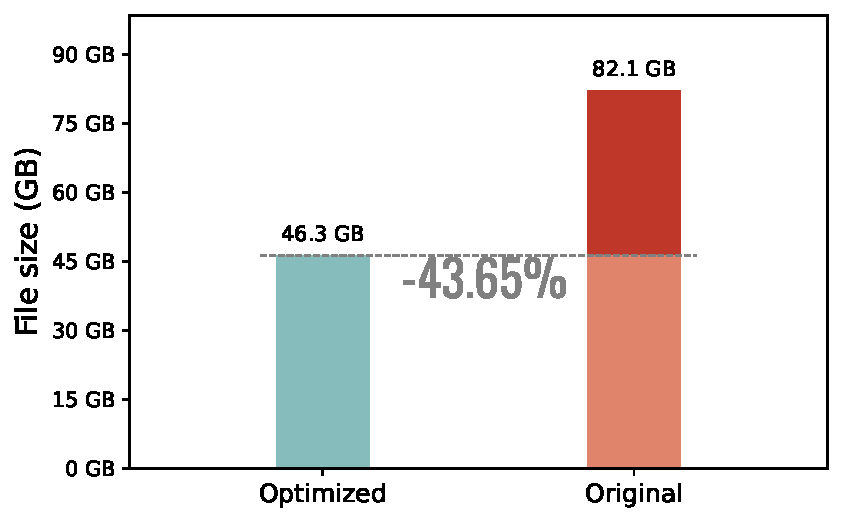
\includegraphics[width=\textwidth]{images/seqdbsize_large.pdf}
      \caption{The amount of space reduction for a 82.1 GB database. The space saving is even higher than smaller databases, reaching $43.65\%$.}
      \label{fig:seqdbsize_large}
    \end{subfigure}
    \caption{\textbf{Effect of \texttt{ASCII}-squeezing method and simplified database index.} We also briefly test the effect of the compression efficiency with respect to the size of the database. The reduction of the indexing overhead is more conspicuous for larger databases.
    If compared with the original \texttt{FASTA} files, the space saving is steadily around $15\%$.}
    \label{fig:ascii-squeezing}
  \end{figure}
  \restoregeometry
\end{figpage}
\pagebreak
\begin{figpage}
  \newgeometry{left=8mm, right=8mm, top=15mm}
  \captionsetup[figure]{width=.8\linewidth}
  \captionsetup[table]{width=.8\linewidth}
  \begin{figure}[t]
    \centering
    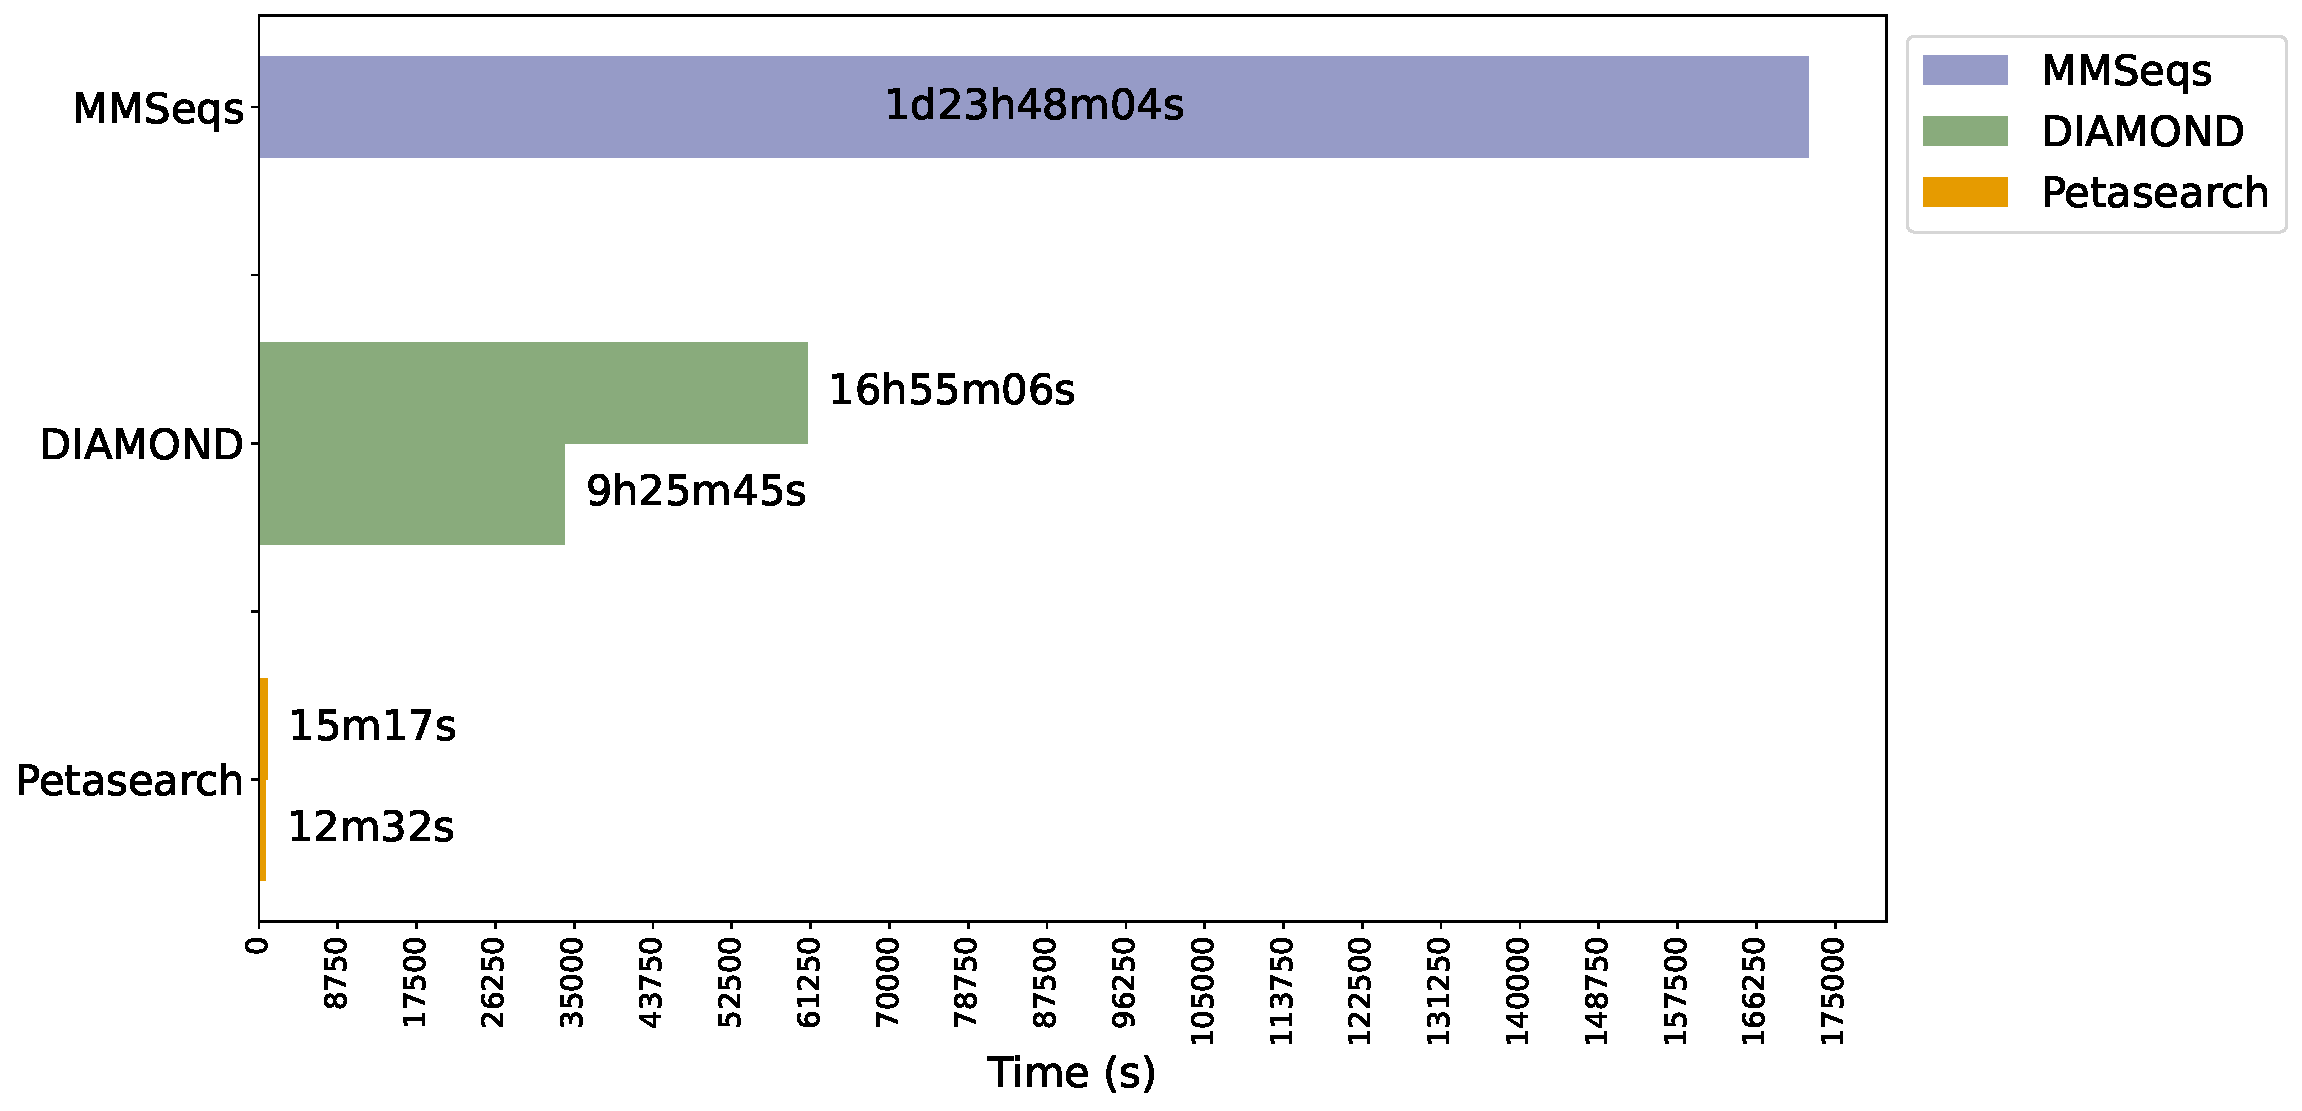
\includegraphics[width=0.8\textwidth]{images/time_benchmark.pdf}
    \caption{\textbf{Visualization of the speed benchmark results.}
      It is clearly shown that the optimization is very effective -- the runtime of \texttt{Petasearch} is almost negligible compared to \texttt{MMseqs2} and \texttt{DIAMOND}.}
    \label{fig:speed}
  \end{figure}
  \begin{table}[]
    \centering
    \begin{tabular}{|c|c|c|l|l|}
      \hline
      \rowcolor[HTML]{5263B5}
      {\color[HTML]{FFFFFF} Name}                                                            &
      {\color[HTML]{FFFFFF} Time}                                                            &
      {\color[HTML]{FFFFFF} Speed up}                                                        &
      \multicolumn{1}{c|}{\cellcolor[HTML]{5263B5}{\color[HTML]{FFFFFF} Special parameters}} &
      \multicolumn{1}{c|}{\cellcolor[HTML]{5263B5}{\color[HTML]{FFFFFF} Notes}}                                                                                                                    \\ \hline
      \rowcolor[HTML]{FFFFFF}
      \cellcolor[HTML]{FFFFFF}                                                               & 12m 32s     & -    & \texttt{--exact-kmer-matching 1} &
      \begin{tabular}[c]{@{}l@{}}Do not generate similar k-mers for query\\ database. \end{tabular}                                                                                                \\ \cline{2-5}
      \rowcolor[HTML]{FFFFFF}
      \multirow{-2}{*}{\cellcolor[HTML]{FFFFFF}petasearch}                                   & 15m 17s     & -    & \texttt{--exact-kmer-matching 0} &
      \begin{tabular}[c]{@{}l@{}} Generate similar k-mers for query datab\\ase. \end{tabular}                                                                                                      \\ \hline
      \rowcolor[HTML]{FFFFFF}
      \cellcolor[HTML]{FFFFFF}                                                               &
      9h 25m 45s                                                                             &
      38x                                                                                    &
      \texttt{--min-score 40 --algo 1}                                                       &
      \begin{tabular}[c]{@{}l@{}}Apply the fast query-indexed algorithm. \\ Did not include the \texttt{makedb} time \end{tabular}                                                                 \\ \cline{2-5}
      \rowcolor[HTML]{FFFFFF}
      \multirow{-2}{*}{\cellcolor[HTML]{FFFFFF}DIAMOND}                                      &
      16h 55m 06s                                                                            &
      68x                                                                                    &
      \texttt{--min-score 40 --algo 0}                                                       &
      \begin{tabular}[c]{@{}l@{}}Use the default sensitive double-indexed \\algorithm.\\ Did not include the \texttt{makedb} time \end{tabular}                                                    \\ \hline
      \rowcolor[HTML]{FFFFFF}
      MMseqs2                                                                                & 47h 48m 04s & 191x & Default params                   & Did not include the \texttt{createdb} time. \\ \hline
    \end{tabular}
    \caption{\textbf{Results of the time benchmark using \texttt{Petasearch}, \texttt{MMseqs2} and \texttt{DIAMOND}.}
      We searched a 2MB query set against a 9.3TB target set (size of the \texttt{FASTA} file including the headers). We prepared a total of 146 target database chunks distributed across 21 NVMe SSDs, 11 of which have 6 chunks and 10 of which have 8 chunks.
      The size of the chunks are evenly distributed. For \texttt{Petasearch}, we repeated the benchmark 10 times to get an average time.
      For \texttt{MMseqs2} and \texttt{DIAMOND}, they were only run once since the time for a full round of search is too long. The parameters and the corresponding explanation of the parameters used in the benchmark were given in the fourth and fifth columns of the table.}
    \label{tab:time_benchmark}
  \end{table}
  \restoregeometry
\end{figpage}
\pagebreak

\begin{figpage}
  \newgeometry{left=8mm, right=8mm}
  \captionsetup[figure]{width=.8\linewidth}
  \begin{figure}
    \centering
    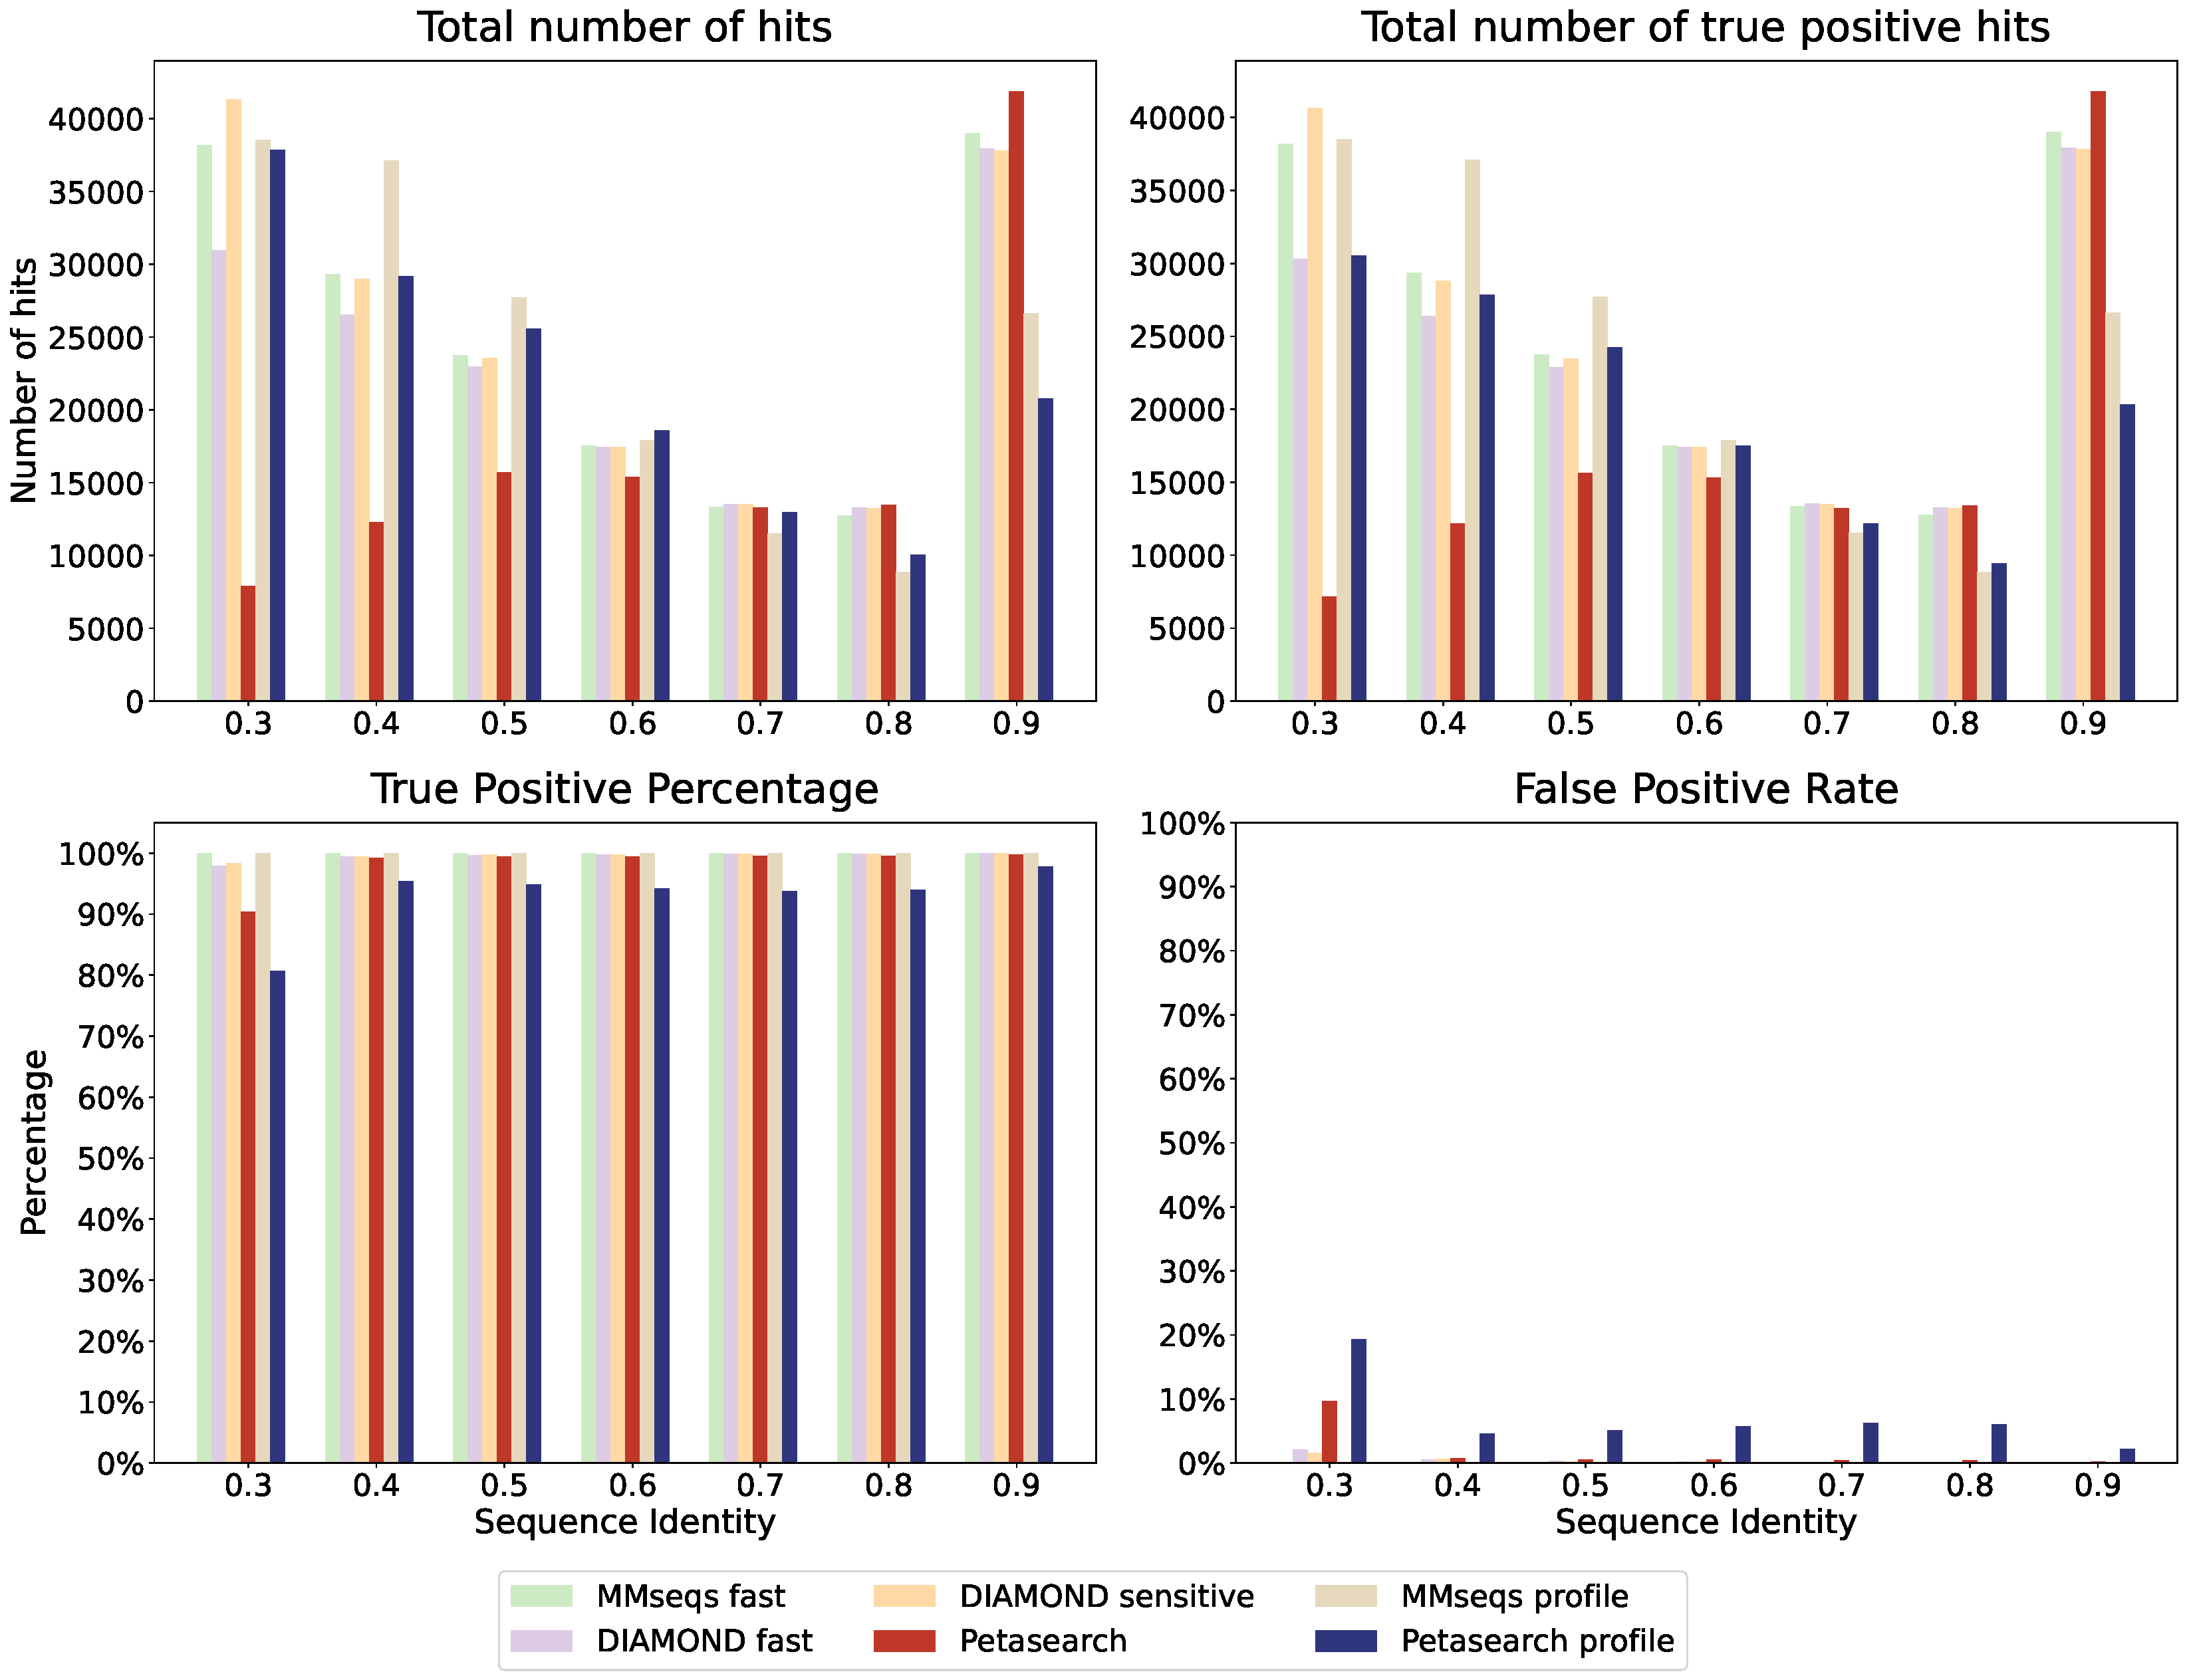
\includegraphics[width=\textwidth]{images/everything.pdf}
    \caption{\textbf{Results of the sensitivity benchmark.} The upper left figure shows the overall hits, the upper right figure shows the total number of true positive hits, the lower left figure shows the true positive rate and the lower right figure shows the false positive rate, each distributed across seven sequence identity buckets. It is clear that the sensitivity of \texttt{Petasearch} is comparable to the state-of-the-art algorithms in sequence identity buckets. For lower sequence identity buckets, the newly added profile search function can compensate for the loss of sensitivity.}
    \label{fig:sensitivity}
  \end{figure}
  \restoregeometry
\end{figpage}
\pagebreak
